\documentclass[11pt]{article}
\usepackage[margin=1in]{geometry}
\usepackage[T1]{fontenc}
\usepackage[utf8]{inputenc}
\usepackage{lmodern}
\usepackage{microtype}
\usepackage{booktabs}
\usepackage{multirow}
\usepackage{tabularx}
\usepackage{array}
\usepackage{amsmath}
\usepackage{amssymb}
\usepackage{mathtools}
\usepackage{bm}
\usepackage{siunitx}
\usepackage{xcolor}
\usepackage{graphicx}
\usepackage{enumitem}
\usepackage{xurl}
\usepackage[colorlinks=true,linkcolor=blue,citecolor=blue,urlcolor=blue]{hyperref}
\usepackage{tikz}
\usepackage{pgfplots}
\pgfplotsset{compat=1.18}
\usetikzlibrary{arrows.meta,positioning,calc,fit,backgrounds,shapes.geometric,decorations.pathreplacing}

\newcommand{\iconmem}{\textbf{DB}}
\newcommand{\iconbrain}{\textbf{AI}}
\newcommand{\iconchip}{\textbf{HW}}
\newcommand{\iconcheck}{\textbf{OK}}
\newcommand{\repo}[1]{\texttt{\nolinkurl{#1}}}
\newcommand{\method}[1]{\textsc{#1}}
\newcommand{\loss}{\mathcal{L}}
\newcommand{\R}{\mathbb{R}}

\title{Breaking the Local Perception Frontier with World-Anchored Foundation Teachers\\
\large A Research Proposal for \texttt{tsqbev-poc}}
\author{tsqbev-poc working proposal}
\date{April 5, 2026}

\begin{document}
\maketitle

\begin{abstract}
The current \texttt{tsqbev-poc} repository has crossed the threshold from ``toy public scaffold'' to
``measured but still weak local control.'' The best trusted local model reaches \texttt{NDS 0.1833}
and \texttt{mAP 0.1814} on \texttt{nuScenes mini\_val}, while the reproduced public
\texttt{BEVFusion} teacher/control reaches \texttt{NDS 0.7072} and \texttt{mAP 0.6730}. This gap is
too large to close with more local query-budget nudges. We propose a new research program centered
on a \emph{world-anchored latent contract}: an efficient \texttt{Sparse4D}-style student, a
\texttt{DINOv3}-conditioned camera branch with \texttt{BEVFormer v2}-style perspective
supervision, dense world-aligned distillation from unrestricted teachers such as
\texttt{BEVFusion}/\texttt{OpenPCDet}, and offline region-support priors from \texttt{SAM 2.1}. We
argue from exact local evidence, the repository's promoted research-memory state, and primary-source
literature that three lessons matter most. First, camera foundation features require a geometry-aware
bridge before they can improve 3D metrics. Second, lane learning should be attached only after the
shared world latent is stable. Third, the control plane for research itself must be official-metric
driven, exact-state aware, and resistant to low-signal branch churn. We define the proposed model,
the distillation objectives, the staged multitask curriculum, the hardware-aware deployment path,
and falsifiable success criteria for the next frontier push.
\end{abstract}

\section{Introduction}
Multimodal 3D perception is currently pulled in two directions. On one side, unrestricted teacher
systems such as \texttt{BEVFusion} and strong LiDAR detectors define practical upper bounds for
public-dataset performance. On the other side, deployable students must survive sparse compute,
limited VRAM, export constraints, and latency budgets. The central question for this repository is
not whether a giant teacher can work; that has already been demonstrated. The question is how to
use frontier teachers and frontier vision priors to move a small student across a real metric
frontier without collapsing deployment viability.

The local evidence is now concrete. The repository's best trusted local control,
\repo{artifacts/research\_v29\_continuation\_v1/research\_loop/summary.json}, reaches
\texttt{NDS 0.1833}, \texttt{mAP 0.1814}, \SI{18.34}{ms} mean latency, and \texttt{40.0}
boxes/sample on \texttt{mini\_val}. The reproduced public teacher ceiling,
\repo{artifacts/bevfusion\_repro/bevfusion\_bbox\_summary.json}, remains far ahead at
\texttt{NDS 0.7072}, \texttt{mAP 0.6730}. The first real \texttt{DINOv3} probe,
\repo{artifacts/foundation\_v3\_dinov3\_teacher\_vits16\_36ep\_v1/epoch022\_probe\_r4/metrics/nuscenes/metrics\_summary.json},
is promising but still below the trusted control at \texttt{NDS 0.1616}, \texttt{mAP 0.1591}. The
naive joint detection+lane branch already failed catastrophically on official detection metrics,
reaching zero on \texttt{mini\_val}; therefore, more naive multitask reruns are not a viable
frontier strategy.

This proposal makes three claims.
\begin{enumerate}[leftmargin=*,itemsep=2pt]
\item The next breakthrough must be \emph{world-aligned}, not just backbone-heavier. This means a
shared latent in world or BEV coordinates that every teacher supervises explicitly.
\item Cross-modal fusion and temporal memory should be separated conceptually. Gated or deformable
cross-attention is the right tool for selective spatial fusion, while selective state-space models
are better treated as later temporal efficiency upgrades rather than immediate substitutes for
spatial alignment.
\item The research lab itself must be a first-class system. Exact memory, semantic retrieval,
official-metric checkpointing, and promotion gates are part of the scientific method here, not just
operator convenience.
\end{enumerate}

\section{Empirical Starting Point}
\begin{table}[t]
\centering
\caption{Exact local starting point for this proposal. All numbers are drawn from repository
artifacts referenced in the text.}
\label{tab:starting-point}
\begin{tabular}{lrrrr}
\toprule
System & Split & NDS & mAP & Notes \\
\midrule
Trusted local control & \texttt{mini\_val} & 0.1833 & 0.1814 & \SI{18.34}{ms}, 40.0 boxes/sample \\
\texttt{DINOv3} probe & \texttt{mini\_val} & 0.1616 & 0.1591 & real signal, not yet a win \\
Naive joint det+lane & \texttt{mini\_val} & 0.0000 & 0.0000 & invalid path \\
Reproduced \texttt{BEVFusion} & \texttt{val} & 0.7072 & 0.6730 & teacher/control ceiling \\
\bottomrule
\end{tabular}
\end{table}

The numbers in Table~\ref{tab:starting-point} imply two things. First, the repository is no longer
blocked by complete model failure. There is a real local control and a real dense teacher ceiling.
Second, the local frontier is not yet close enough to justify incrementalism. The gap to the teacher
is still \(\Delta\text{NDS}\approx0.5239\), which is far too large to be explained by scheduler
tweaks or slight query-count changes.

The promoted memory build,
\repo{artifacts/memory/sync\_manifest.json}, reinforces the same diagnosis. It indexes \texttt{65}
high-signal facts and explicitly surfaces repeated rabbit holes such as
\repo{incremental\_progress}, \repo{schedule\_checkpoint\_drift}, and
\repo{vehicle\_emergence\_failure}. This is the empirical reason we should not restart a broad
local loop until the next branch is hypothesis-tight.

\section{Literature-Grounded Design Principles}
\paragraph{Foundation camera features require a geometry bridge.}
\texttt{DINOv3} shows that large-scale self-supervised vision backbones can retain strong dense
transfer features, but this does not automatically solve 3D localization \cite{dinov3}. The local
\texttt{DINOv3} probe confirms the same lesson: a stronger image backbone alone is not enough.
\texttt{BEVFormer v2} makes the relevant move by supervising the image-to-BEV bridge in perspective
space \cite{bevformerv2}. This is the first principle behind the proposal.

\paragraph{World-aligned distillation beats local heuristics.}
\texttt{DistillBEV} and \texttt{UniDistill} argue that camera students improve more reliably when
they are supervised in a BEV or world-aligned space by stronger teachers \cite{distillbev,unidistill}.
This is the second principle: the student should be taught the world, not just the final box list.

\paragraph{Region support is a teacher-side problem first.}
\texttt{SAM 2.1} is valuable here because it can turn sparse prompts, boxes, or tracked cues into
dense support masks with memory across frames \cite{sam2}. The right use is offline or asynchronous
teacher-side support generation, not replacing the deployable perception trunk.

\paragraph{Fusion and temporal memory should be separated.}
Gated cross-attention is a selective \emph{external lookup} mechanism, while Mamba-like selective
SSMs are \emph{internal temporal memory} mechanisms \cite{flamingo,mamba}. Conflating them is a
category error. We therefore use gated or deformable fusion for spatial cross-modal alignment now,
and treat temporal SSMs as a later optimization path if and only if the spatial/world latent is
already winning.

\paragraph{Lane learning should be attached through a vector head, not loss soup.}
\texttt{MapTRv2} supports staged vector-map learning on top of a world-aligned representation
\cite{maptrv2}. The failed naive joint branch in this repo is direct evidence that simply adding
lane loss to the student is not enough.

\paragraph{Efficiency comes after the frontier branch is real.}
MIT HAN Lab systems work such as \texttt{EfficientViT}, \texttt{OFA}, \texttt{AMC}, \texttt{HAQ},
\texttt{AWQ}, \texttt{Quest}, and \texttt{XAttention} is highly relevant, but mostly as a second
step: once the perception path is winning, use hardware-aware compression or sparse kernels to make
it cheap \cite{efficientvit,ofa,amc,haq,awq,quest,xattention}. NVIDIA's TensorRT-LLM and Model
Optimizer live in the same category for this repo \cite{trtllm,modelopt}. They are not the first
fix for a weak world model.

\section{Proposed System: World-Anchored Foundation Teachers}
\subsection{High-level architecture}
\begin{figure*}[t]
\centering
\resizebox{\linewidth}{!}{%
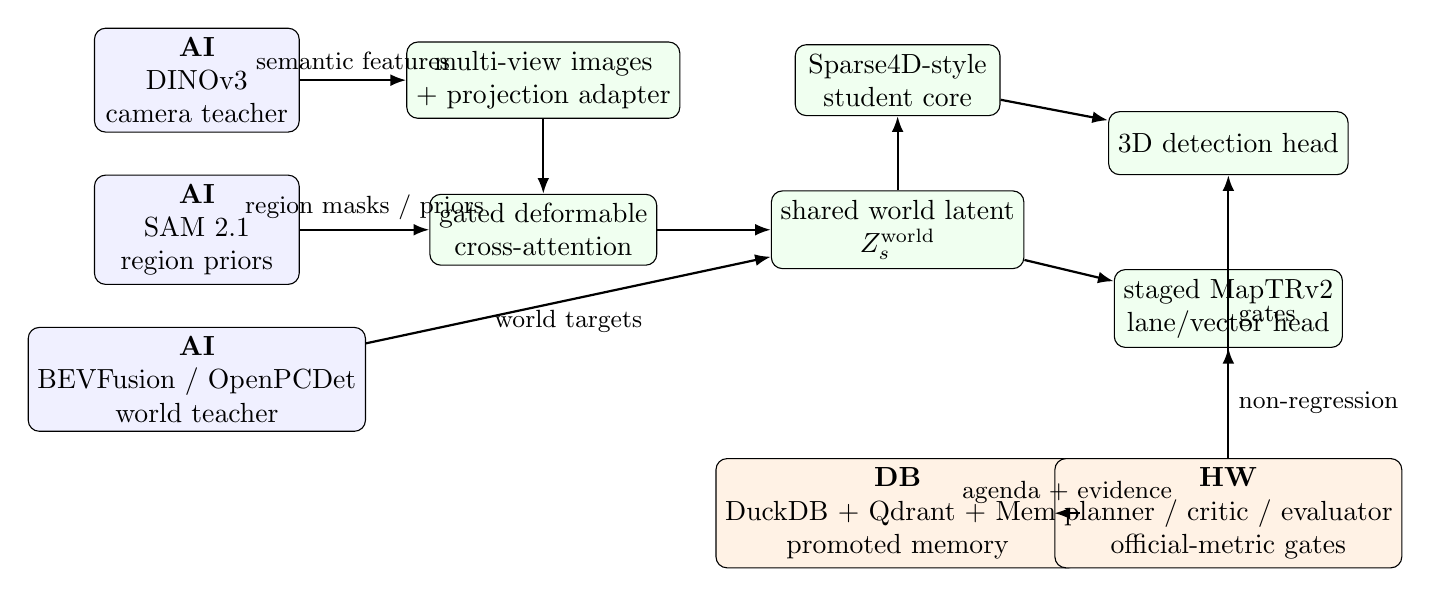
\begin{tikzpicture}[
  box/.style={draw, rounded corners, align=center, minimum width=2.6cm, minimum height=8mm, fill=white},
  teacher/.style={box, fill=blue!6},
  student/.style={box, fill=green!6},
  control/.style={box, fill=orange!10},
  arr/.style={-{Latex[length=2mm]}, thick},
  note/.style={align=center, font=\small}
]
\node[teacher] (dino) at (0,3.2) {\iconbrain\\DINOv3\\camera teacher};
\node[teacher] (sam) at (0,1.3) {\iconbrain\\SAM 2.1\\region priors};
\node[teacher] (bevfusion) at (0,-0.6) {\iconbrain\\BEVFusion / OpenPCDet\\world teacher};

\node[student] (cams) at (4.4,3.2) {multi-view images\\+ projection adapter};
\node[student] (cross) at (4.4,1.3) {gated deformable\\cross-attention};
\node[student] (world) at (8.9,1.3) {shared world latent\\$Z^{\text{world}}_s$};
\node[student] (sparse4d) at (8.9,3.2) {Sparse4D-style\\student core};
\node[student] (det) at (13.1,2.4) {3D detection head};
\node[student] (lane) at (13.1,0.3) {staged MapTRv2\\lane/vector head};

\node[control] (mem) at (8.9,-2.3) {\iconmem\\DuckDB + Qdrant + Mem0\\promoted memory};
\node[control] (ctrl) at (13.1,-2.3) {\iconchip\\planner / critic / evaluator\\official-metric gates};

\draw[arr] (dino) -- node[above, note] {semantic features} (cams);
\draw[arr] (sam) -- node[above, note] {region masks / priors} (cross);
\draw[arr] (bevfusion) -- node[below, note] {world targets} (world);
\draw[arr] (cams) -- (cross);
\draw[arr] (cross) -- (world);
\draw[arr] (world) -- (sparse4d);
\draw[arr] (sparse4d) -- (det);
\draw[arr] (world) -- (lane);
\draw[arr] (mem) -- node[above, note] {agenda + evidence} (ctrl);
\draw[arr] (ctrl) -- node[right, note] {gates} (det);
\draw[arr] (ctrl) -- node[right, note] {non-regression} (lane);
\end{tikzpicture}}
\caption{Proposal overview. Heavy teachers supervise a shared world latent rather than directly
replacing the deployable student. The control plane uses exact memory and official-metric gates to
prevent low-signal branch churn.}
\label{fig:proposal}
\end{figure*}

The central design is shown in Figure~\ref{fig:proposal}. We propose a \textbf{shared world latent
contract}: every expensive teacher supervises the same student latent in world or BEV coordinates,
instead of each teacher attaching ad hoc local losses to separate branches.

The runtime student remains a \texttt{Sparse4D}-style sparse temporal model \cite{sparse4d}. The
camera branch is strengthened with \texttt{DINOv3} priors and a learned projection adapter. A
gated deformable cross-attention block fuses camera support into the world latent. The dense
teacher side supplies three different kinds of supervision:
\begin{enumerate}[leftmargin=*,itemsep=2pt]
\item semantic camera priors from \texttt{DINOv3},
\item region support from \texttt{SAM 2.1},
\item world-aligned geometry and BEV targets from \texttt{BEVFusion} or strong LiDAR teachers.
\end{enumerate}

\subsection{Student-side fusion}
Let \(q_i \in \R^d\) be the \(i\)-th sparse query with a projected multi-view reference point
\(\pi_h(\hat b_i)\) in image \(h\). Let \(F_h \in \R^{C\times H \times W}\) be the projected
\texttt{DINOv3}-conditioned feature map for view \(h\). The fused query update is
\begin{equation}
\tilde q_i
= q_i
+ g_i \odot
\sum_{h=1}^{N_v}\sum_{k=1}^{K}
\alpha_{ihk}\,W_v\,F_h\!\left(\pi_h(\hat b_i)+\Delta p_{ihk}\right),
\qquad
g_i = \sigma(W_g q_i).
\label{eq:gated-cross}
\end{equation}
Equation~\eqref{eq:gated-cross} encodes the key distinction from the KB: cross-attention is the
right mechanism for \emph{whether and where} to read external evidence, not for long-horizon
temporal carry.

\subsection{Perspective supervision}
To make the image-to-world bridge geometry-aware, we add a \texttt{BEVFormer v2}-style
perspective-space auxiliary signal. Let \(P_h(\tilde q)\) be a view-conditioned projector and
\(T_h^{\text{persp}}\) a teacher target in perspective space. Then
\begin{equation}
\loss_{\text{persp}}
=
\sum_{h=1}^{N_v}
\left\|
M_h \odot \left(P_h(\tilde q)-T_h^{\text{persp}}\right)
\right\|_1,
\label{eq:persp}
\end{equation}
where \(M_h\) masks valid view support.

\subsection{World-aligned distillation}
Let \(Z_s^{\text{world}}\) and \(Z_t^{\text{world}}\) be the student and teacher world latents,
with small alignment heads \(A_s, A_t\). We use
\begin{equation}
\loss_{\text{bev}}
=
\left\|
M^{\text{fg}} \odot \left(A_s(Z_s^{\text{world}})-A_t(Z_t^{\text{world}})\right)
\right\|_1
\end{equation}
for dense BEV or world-latent alignment, and
\begin{equation}
\loss_{\text{quality}}
=
\mathrm{VFL}(s_s, q_t)
+ \lambda_{\text{box}}
\left(
\|c_s-c_t\|_1 + \|d_s-d_t\|_1 + \mathrm{GIoU}(b_s,b_t)
\right),
\label{eq:quality}
\end{equation}
where \(q_t\) is a quality-aware teacher target, \(s_s\) is the student ranking score, and
\((c,d,b)\) denote center, dimensions, and box geometry.

\subsection{Region-support distillation from \texttt{SAM 2.1}}
Let \(M_{\text{sam}}\) be a teacher region prior warped into the world grid by \(\mathcal{W}\). The
student predicts occupancy or support logits \(H_{\text{occ}}(Z_s^{\text{world}})\), giving
\begin{equation}
\loss_{\text{occ}}
=
\mathrm{BCE}\!\left(
\sigma\!\left(H_{\text{occ}}(Z_s^{\text{world}})\right),
\mathcal{W}(M_{\text{sam}})
\right).
\label{eq:occ}
\end{equation}
This loss exists to preserve object support and foreground structure that box-only supervision
cannot preserve reliably.

\subsection{Staged lane integration}
We do \emph{not} attach lane learning to the student by default. Instead,
\begin{equation}
\loss
=
\loss_{\text{det}}
\,+\,\lambda_{\text{persp}}\loss_{\text{persp}}
\,+\,\lambda_{\text{bev}}\loss_{\text{bev}}
\,+\,\lambda_{\text{quality}}\loss_{\text{quality}}
\,+\,\lambda_{\text{occ}}\loss_{\text{occ}}
\,+\,\mathbf{1}[r_{\text{det}}\ge\tau]\lambda_{\text{lane}}\loss_{\text{lane}},
\label{eq:stage}
\end{equation}
where \(r_{\text{det}}\) is the current official detection non-regression signal and \(\tau\) is the
promotion threshold. This enforces the repo lesson that lane is only allowed onto the shared latent
after detection is stable.

\section{Research Control Plane}
\begin{figure}[t]
\centering
\resizebox{0.95\linewidth}{!}{%
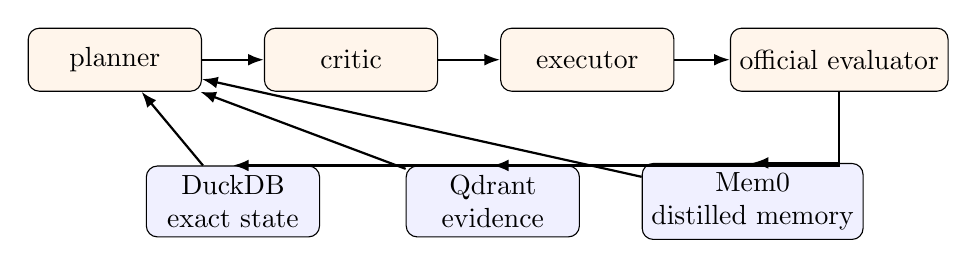
\begin{tikzpicture}[
  box/.style={draw, rounded corners, align=center, minimum width=2.2cm, minimum height=8mm, fill=white},
  stage/.style={box, fill=orange!8},
  mem/.style={box, fill=blue!6},
  arr/.style={-{Latex[length=2mm]}, thick}
]
\node[stage] (planner) at (0,1.8) {planner};
\node[stage] (critic) at (3.0,1.8) {critic};
\node[stage] (executor) at (6.0,1.8) {executor};
\node[stage] (evaluator) at (9.2,1.8) {official evaluator};
\node[mem] (duckdb) at (1.5,0) {DuckDB\\exact state};
\node[mem] (qdrant) at (4.8,0) {Qdrant\\evidence};
\node[mem] (mem0) at (8.1,0) {Mem0\\distilled memory};

\draw[arr] (planner) -- (critic);
\draw[arr] (critic) -- (executor);
\draw[arr] (executor) -- (evaluator);
\draw[arr] (duckdb) -- (planner);
\draw[arr] (qdrant) -- (planner);
\draw[arr] (mem0) -- (planner);
\draw[arr] (evaluator.south) |- (duckdb.north);
\draw[arr] (evaluator.south) |- (qdrant.north);
\draw[arr] (evaluator.south) |- (mem0.north);
\end{tikzpicture}}
\caption{Research control plane. The proposal treats exact state, semantic evidence, and distilled
memory as scientific infrastructure rather than optional tooling.}
\label{fig:control}
\end{figure}

The repo has already learned that automation without exact-state gates is not enough. The current
memory layer now maintains a promoted DuckDB-backed exact catalog, a Qdrant evidence layer, and an
optional Mem0 distilled layer. The proposal therefore uses the control plane in
Figure~\ref{fig:control} as part of the scientific process:
\begin{enumerate}[leftmargin=*,itemsep=2pt]
\item \textbf{Planner}: reads exact frontier state and reranked evidence.
\item \textbf{Critic}: rejects low-ROI branches, repeated rabbit holes, or uncontrolled multitask
coupling.
\item \textbf{Executor}: runs only bounded experiments.
\item \textbf{Evaluator}: selects checkpoints by official metrics, not by loss.
\end{enumerate}

Promotion is conditioned on
\begin{equation}
\Delta_{\text{promote}}
=
\mathbf{1}[\text{NDS}_{\text{new}} > \text{NDS}_{\text{ctrl}}]
\cdot
\mathbf{1}[\text{mAP}_{\text{new}} \ge \text{mAP}_{\text{ctrl}} - \epsilon]
\cdot
\mathbf{1}[\ell_{\text{lat}} \le \ell_{\max}]
\cdot
\mathbf{1}[\text{geom sanity}],
\label{eq:promote}
\end{equation}
where \(\epsilon\) is a small tolerated regression band and ``geom sanity'' includes export validity,
boxes/sample, and physically plausible box ranges.

\section{Staged Experimental Program}
\begin{table*}[t]
\centering
\caption{Proposed staged program. Each stage has a hard falsifier so the loop cannot drift
indefinitely.}
\label{tab:stages}
\begin{tabularx}{\linewidth}{l l X X}
\toprule
Stage & Goal & Proposed mechanism & Falsifier / gate \\
\midrule
S0 & hold a trusted control & keep the current \texttt{v29} line as the baseline & any new branch must report official metrics against it \\
S1 & stronger camera-to-world bridge & \texttt{DINOv3} + projection adapter + perspective supervision & if official \texttt{mini\_val} stays below control after teacher distillation, stop backbone-only work \\
S2 & stronger world supervision & \texttt{BEVFusion/OpenPCDet} BEV distillation + quality targets + \texttt{SAM 2.1} region priors & if geometry/export does not improve, stop adding more teacher loss terms blindly \\
S3 & stable lane integration & staged \texttt{MapTRv2} vector head with non-regression gate & if detection drops beyond tolerance, revert to frozen shared trunk \\
S4 & efficiency and deployment & activation checkpointing, dynamic VRAM fit, then \texttt{EfficientViT}/\texttt{OFA}/\texttt{AMC}/\texttt{HAQ}/\texttt{AWQ} & only start after S1/S2 produce a real metric win \\
\bottomrule
\end{tabularx}
\end{table*}

The immediate frontier work should stop after S2 if it does not beat the trusted control. In that
case the repo should pivot architecture family again rather than continuing local tweaks.

\section{Expected Breakthrough Mechanism}
The proposal's central new hypothesis is this:
\begin{quote}
\textbf{The smallest deployable student can break the local frontier only if all heavy teachers
supervise the \emph{same world latent}, while the camera branch is explicitly taught how image-space
semantics map into world-space geometry.}
\end{quote}

This is more specific than ``use a better backbone'' and more disciplined than ``try all tricks.''
It implies the following unique synthesis:
\begin{enumerate}[leftmargin=*,itemsep=2pt]
\item \texttt{DINOv3} is not the solution by itself; it is the semantic teacher for the camera
branch.
\item \texttt{BEVFormer v2}-style perspective supervision is the bridge that tells the camera
branch where 3D cues live.
\item \texttt{BEVFusion}/\texttt{OpenPCDet} distillation is the geometry teacher for the shared
world latent.
\item \texttt{SAM 2.1} is the region-support teacher that preserves object support and occupancy.
\item Lane enters only after the shared latent proves itself under official detection metrics.
\end{enumerate}

\section{Why Not Other Directions First?}
\paragraph{Why not Mamba first?}
The KB explicitly distinguishes fusion from temporal memory. Mamba-style SSMs may eventually
replace or compress temporal attention, but they do not solve the current image-to-world bridge
problem \cite{mamba}. Starting there would be a category error.

\paragraph{Why not MoE first?}
MoE is a teacher-side or control-plane efficiency tool unless the student already needs more
capacity than dense compute can provide. The repo is not there yet.

\paragraph{Why not Alpamayo or Cosmos as the perception trunk?}
These systems belong in reasoning, scenario analysis, and teacher-side generation roles, not as the
immediate 3D localization trunk \cite{alpamayo,cosmosreason,cosmospredict}.

\paragraph{Why not more naive joint detection+lane training?}
Because the repo already has direct counter-evidence: the current joint path can look acceptable on
loss and still collapse detection to zero on official metrics.

\section{Hardware and Deployment Plan}
The proposal keeps deployment constraints explicit:
\begin{enumerate}[leftmargin=*,itemsep=2pt]
\item activation checkpointing for the heavy camera projector blocks,
\item automatic VRAM-fit policy for batch size and accumulation,
\item deformable or sparse fusion before any dense attention expansion,
\item compression and quantization only after the new branch wins on metrics.
\end{enumerate}

This is where \texttt{EfficientViT}, \texttt{OFA}, \texttt{AMC}, \texttt{HAQ}, and \texttt{AWQ}
enter the story \cite{efficientvit,ofa,amc,haq,awq}. They are later-stage accelerants, not the
first-order frontier move.

\section{Conclusion}
The repository is ready for a harder and more coherent phase. The memory layer is now promoted and
queryable. The knowledge base is broad enough to support a real frontier proposal. The correct next
step is not a larger random sweep; it is a world-anchored, teacher-coalition student that makes
every heavy model pay rent in the same shared latent. If that branch fails to beat the trusted
control, the repo should pivot architecture family again on explicit evidence rather than hiding the
failure inside another low-signal loop.

\begin{thebibliography}{99}

\bibitem{dinov3}
\emph{DINOv3}. Meta AI project page and official code, 2026.
\url{https://ai.meta.com/resources/models-and-libraries/dinov3-downloads/},
\url{https://github.com/facebookresearch/dinov3}

\bibitem{sam2}
\emph{SAM 2: Segment Anything in Images and Videos}. arXiv:2408.00714, 2024.
\url{https://arxiv.org/abs/2408.00714},
\url{https://github.com/facebookresearch/sam2}

\bibitem{bevformerv2}
\emph{BEVFormer v2: Adapting Modern Image Backbones to Birds-Eye-View Recognition via Perspective
Supervision}. CVPR 2023.
\url{https://openaccess.thecvf.com/content/CVPR2023/papers/Yang_BEVFormer_v2_Adapting_Modern_Image_Backbones_to_Birds-Eye-View_Recognition_via_CVPR_2023_paper.pdf}

\bibitem{sparse4d}
\emph{Sparse4D: Multi-view 3D Object Detection with Sparse Spatial-Temporal Fusion}. arXiv:2211.12413, 2022.
\url{https://arxiv.org/abs/2211.12413}

\bibitem{distillbev}
\emph{DistillBEV: Boosting Multi-Camera 3D Object Detection with Cross-Modal Knowledge Distillation}. ICCV 2023.
\url{https://openaccess.thecvf.com/content/ICCV2023/html/Wang_DistillBEV_Boosting_Multi-Camera_3D_Object_Detection_with_Cross-Modal_Knowledge_Distillation_ICCV_2023_paper.html}

\bibitem{unidistill}
\emph{UniDistill: A Universal Cross-Modality Knowledge Distillation Framework for 3D Object Detection in Bird's-Eye View}. CVPR 2023.
\url{https://openaccess.thecvf.com/content/CVPR2023/html/Zhou_UniDistill_A_Universal_Cross-Modality_Knowledge_Distillation_Framework_for_3D_Object_CVPR_2023_paper.html}

\bibitem{maptrv2}
\emph{MapTRv2: Structured Modeling and Learning for Online Vectorized HD Map Construction}. arXiv:2308.05736, 2023.
\url{https://arxiv.org/abs/2308.05736}

\bibitem{flamingo}
\emph{Flamingo: a Visual Language Model for Few-Shot Learning}. arXiv:2204.14198, 2022.
\url{https://arxiv.org/abs/2204.14198}

\bibitem{deformabledetr}
\emph{Deformable DETR: Deformable Transformers for End-to-End Object Detection}. arXiv:2010.04159, 2020.
\url{https://arxiv.org/abs/2010.04159}

\bibitem{blip2}
\emph{BLIP-2: Bootstrapping Language-Image Pre-training with Frozen Image Encoders and Large Language Models}. arXiv:2301.12597, 2023.
\url{https://arxiv.org/abs/2301.12597}

\bibitem{mamba}
\emph{Mamba: Linear-Time Sequence Modeling with Selective State Spaces}. arXiv:2312.00752, 2023.
\url{https://arxiv.org/abs/2312.00752}

\bibitem{byot}
\emph{Be Your Own Teacher: Improve the Performance of Convolutional Neural Networks via Self Distillation}. ICCV 2019.
\url{https://openaccess.thecvf.com/content_ICCV_2019/html/Zhang_Be_Your_Own_Teacher_Improve_the_Performance_of_Convolutional_Neural_ICCV_2019_paper.html}

\bibitem{dml}
\emph{Deep Mutual Learning}. CVPR 2018.
\url{https://openaccess.thecvf.com/content_cvpr_2018/html/Zhang_Deep_Mutual_Learning_CVPR_2018_paper.html}

\bibitem{efficientvit}
\emph{EfficientViT: Multi-Scale Linear Attention for High-Resolution Dense Prediction}. arXiv:2205.14756, 2022.
\url{https://arxiv.org/abs/2205.14756}

\bibitem{ofa}
\emph{Once-for-All: Train One Network and Specialize it for Efficient Deployment}. ICLR 2020.
\url{https://arxiv.org/abs/1908.09791}

\bibitem{amc}
\emph{AMC: AutoML for Model Compression and Acceleration on Mobile Devices}. ECCV 2018.
\url{https://arxiv.org/abs/1802.03494}

\bibitem{haq}
\emph{HAQ: Hardware-Aware Automated Quantization with Mixed Precision}. CVPR 2019.
\url{https://hanlab18.mit.edu/projects/haq/papers/haq_arxiv.pdf}

\bibitem{awq}
\emph{AWQ: Activation-aware Weight Quantization for LLM Compression and Acceleration}. MLSys 2024.
\url{https://arxiv.org/abs/2306.00978}

\bibitem{quest}
\emph{Quest: Query-aware Sparsity for Efficient Long-Context LLM Inference}. arXiv:2406.10774, 2024.
\url{https://arxiv.org/abs/2406.10774}

\bibitem{xattention}
\emph{XAttention: Block Sparse Attention with Antidiagonal Scoring}. arXiv:2503.16428, 2025.
\url{https://arxiv.org/abs/2503.16428}

\bibitem{alpamayo}
\emph{NVIDIA DRIVE Alpamayo}. NVIDIA DRIVE project page, 2026.
\url{https://developer.nvidia.com/drive/alpamayo}

\bibitem{cosmosreason}
\emph{Cosmos-Reason2}. NVIDIA Cosmos code release, 2026.
\url{https://github.com/nvidia-cosmos/cosmos-reason2}

\bibitem{cosmospredict}
\emph{Cosmos-Predict2.5}. NVIDIA Cosmos code release, 2026.
\url{https://github.com/nvidia-cosmos/cosmos-predict2.5}

\bibitem{modelopt}
\emph{NVIDIA Model Optimizer}. NVIDIA repository, 2026.
\url{https://github.com/NVIDIA/Model-Optimizer}

\bibitem{trtllm}
\emph{TensorRT-LLM}. NVIDIA repository, 2026.
\url{https://github.com/NVIDIA/TensorRT-LLM}

\bibitem{bevfusion}
\emph{BEVFusion}. MIT HAN Lab repository, 2026.
\url{https://github.com/mit-han-lab/bevfusion}

\bibitem{openpcdet}
\emph{OpenPCDet}. OpenMMLab repository, 2026.
\url{https://github.com/open-mmlab/OpenPCDet}

\end{thebibliography}

\end{document}
